 \documentclass{article}
 % 3 næste linjer skal med får at vi kan skrive specialtegn såsom æ, ø og å. 
  \usepackage[T1]{fontenc}
  \usepackage[UTF8]{inputenc}
  \usepackage{lmodern}
  \usepackage{graphicx}

  
  \begin{document}
  
  \part*{BDSA --> OOAD \linebreak A Calendar system}
  
  \paragraph{Revision history} \mbox{}  
  
  \begin{table}[ht]
    \begin{tabular}{|p{35pt}|p{50pt}|p{150pt}|p{75pt}|}
        \hline
        Version & Date &
        Description & 
        Author         
        \\ \hline
        01.00.00 & 04-09-2012 & 
        First draft. The document fulfill the requrements for assignemt A36 - PART I &
        Nicolai Krüger 
        \\ \hline        
        01.01.00 & 18-09-2012 & 
        Added Revision history table. Started writing in english (future writing must be in english) - translation of the first version is yet to be done. & 
        Nicolai Krüger              
        \\ \hline
        01.01.01 & 04-09-2012 &
        Changed the titel of the document. \linebreak
        Removed the "use case ends" filed in the Use cases. &
        Nicolai Krüger
        \\ \hline
    \end{tabular}
\end{table}
  
  \paragraph{Vision} \mbox{} 
  
  Programmet skal fungere på en sådan måde, at det skal være muligt at anvende uden brug af musen. Det skal kunne anvendes uden bruge af mange genveje og lignede, men derimod via enkelte essentielle knapper. 
Samtidig skal programmet fungere på touch- og mobilenheder.
  
   \paragraph{Use Cases}
   \begin{itemize}
   \item Opret begivenhed
   	\begin{itemize}
   	\item En bruger begynder at skrive en titel til deres begivenhed og/eller en dato
   	\item Systemet viser både en live-search ud fra titel og dato. Desuden viser systemet også også en "ny begivenhed" formular - dato vil her blive udfyldt hvis brugeren skriver en dato.
   	
   	\item Brugeren at udfylde formularen så meget som der han/ønsker og vælger opret.
   	\item Systemet gemmer aftalen og synkronisere med eventuelle webservere.
   	\item Brugeren får vist den pågældende aftale
   	\item Brugeren får vist hele kalenderen (i forhold til det de fik vist før - dag, uge eller måned) med den pågældende aftale markeret.
   	\item Use case slutter
   	\end{itemize}
   \item Slet begivenhed
   \begin{itemize}
   	\item En bruger begynder at skrive en titel på begivenheden og/eller en dato
   	\item Systemet viser både en live-search ud fra titel og dato. Desuden viser systemet også også en "ny begivenhed" formular - dato vil her blive udfyldt hvis brugeren skriver en dato.
   	\item Brugeren navigere hen til den aftale der ønskes slettet med piletasterne, og trykker på "Delete"
   	\item Systemet sletter aftalen og synkronisere med eventuelle webservere.
   	\item Brugeren får vist hele kalenderen (i forhold til det de fik vist før - dag, uge eller måned)
   	\end{itemize}
   \item Redigere en begivenhed
    \begin{itemize}
   	\item En bruger begynder at skrive en titel på begivenheden og/eller en dato
   	\item Systemet viser både en live-search ud fra titel og dato. Desuden viser systemet også også en "ny begivenhed" formular - dato vil her blive udfyldt hvis brugeren skriver en dato.
   	\item Brugeren navigere hen til den aftale der ønskes redigeret med piletasterne, og trykker "Enter"
   	\item Systemet åbner aftalen, med samtlige felter som værende redigerbare.
   	\item Brugeren redigere de dele af begivenheden som skal redigeres, og gemmer aftalen igen.
   	\item Systemet gemmer aftalen og synkronisere med eventuelle webservere.
   	\item Brugeren får vist hele kalenderen (i forhold til det de fik vist før - dag, uge eller måned) med den pågældende aftale markeret.
   	\end{itemize}
   
   \item Skift visning
   \begin{itemize}
   \item Brugeren navigere op til menuen med 4 knapper - "Dag", "Uge", "Måned" og "Indstillinger"
   \item Brugeren markere en af de 3 første knapper og trykker "enter"
   \item Systemet skifter visning af kalenderen i forhold til hvad der er trykket
   \end{itemize}
   \item Tilføje kalendere (f.eks. hotmail eller gmail)
   \begin{itemize}
   \item Brugeren navigere op til menuen med 4 knapper - "Dag", "Uge", "Måned" og "Indstillinger"
   \item Brugeren markere den sidste knap og trykker "enter"
   \item Systemet viser en liste med indstillings muligheder
   \item Brugeren vælger "Tilføj kalender"
   \item Systemet viser en formular
   \item Brugeren indtaster url til den ønskede kalenders ICS-fil, og udfylder resten af formularen og trykker "enter"
   \item Systemet forsøger at tilfå kalenderen
   \item Systemet henter data fra den nye kalender
   \item Brugeren får vist hele kalenderen (i forhold til det de fik vist før - dag, uge eller måned)
   \end{itemize}
   \item Fjern kalender
   \begin{itemize}
   \item Brugeren navigere op til menuen med 4 knapper - "Dag", "Uge", "Måned" og "Indstillinger"
   \item Brugeren markere den sidste knap og trykker "enter"
   \item Systemet viser en liste med indstillings muligheder
   \item Brugeren vælger "Slet kalender"
   \item Systemet viser en liste over kalendere som systemet henter data fra
   \item Brugeren markere den kalender som ønskes slettes og trykker "enter"
   \item Systemet beder brugeren om at bekræfte sletningen
   \item Brugeren markere "Bekræft sletning" og trykker "enter"
   \item Systemet fjerne alle relationer til kalenderen
   \item Brugeren får vist hele kalenderen (i forhold til det de fik vist før - dag, uge eller måned)
   \end{itemize}
   \item Rediger kalender
   \begin{itemize}
   \item Brugeren navigere op til menuen med 4 knapper - "Dag", "Uge", "Måned" og "Indstillinger"
   \item Brugeren markere den sidste knap og trykker "enter"
   \item Systemet viser en liste med indstillings muligheder
   \item Brugeren vælger rediger kalender
   \item Systemet viser en liste over kalendere som systemet henter data fra
   \item Brugeren markere den kalender som ønskes ændret og trykker "enter"
   \item Systemet viser en formular med udfyldte felter i forhold til den valgte kalender
   \item Brugeren ændre de felter som ønskes ændret, markere "gem" knapper og trykker "enter"
   \item Systemet opdatere med de nye informationer
   \item Brugeren får vist hele kalenderen (i forhold til det de fik vist før - dag, uge eller måned)
   \end{itemize}
   \end{itemize}
   
   \newpage 
   \paragraph{Use Case UML Diagrams} \mbox{}

   
   \begin{figure}[h]
\caption{}   
   \centering
   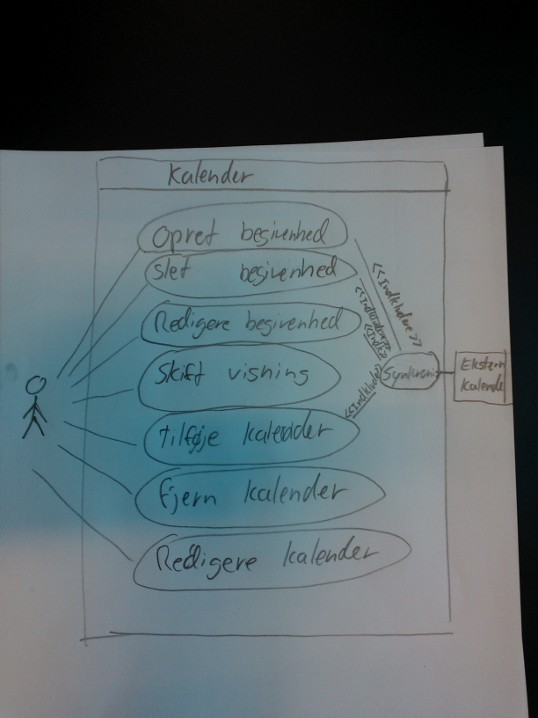
\includegraphics[scale=1.5]{WP_000143.jpg}
   \end{figure}
   
   \paragraph{Glossary} \mbox{}
\subparagraph{Begivenhed} \mbox{}

En begivenhed repræsentere en hver form for opslag i kalenderen. Aftaler, noter, arrangementer, osv. \\
Det er kort sagt den eneste ting der kan slås op, og ses i kalenderen.


   
   \paragraph{Supplementary Requirements (FURPS+)} \mbox{}
   \subparagraph{Functionality} \mbox{}
   
   \subparagraph{Error Handling} \mbox{}
   
   Alle former for fejl og exceptions, skal håndteres efter en på forhånd defineret fejlhåndterings-strategi.
   \subparagraph{Usability} \mbox{}
   
   Det skal være muligt, at anvende kalenderen uden brug af musen og kun ved hjælp af få taster.
   \subparagraph{Reliabilty} \mbox{}
   
   Kalenderen skal fungerer på en sådan måde, at den er stabil. Og hvis der skulle forekomme nedbrud, så skal kalenderen genstarte af sig selv og derved være til minimal gene for brugeren.
   \subparagraph{Performance} \mbox{}
   
   Der er ingen særlige krav til performance, udover at det skal køre flydende, som det kan forventes fra et kalendersystem i dag.
   \subparagraph{Suportability} \mbox{}
   
   
   
   
  \end{document}
